\documentclass[a4paper,11pt,notitlepage,fullpage]{article}
%\documentclass{report}

\usepackage{fullpage}
\usepackage[utf8]{inputenc}
%\usepackage[ngerman]{babel}
%\usepackage[english]{babel}
\usepackage{amsmath}
\usepackage{amssymb}
\usepackage{latexsym}
\usepackage{mathtools}
\usepackage{listings}
\usepackage{bbm}
%\usepackage{algorithm}
%\usepackage{algpseudocode}
\usepackage{graphicx}
\usepackage{booktabs}
\usepackage{hhline}
\usepackage{amsthm}
\usepackage{cite}
\usepackage{wrapfig}
\usepackage{hyperref}
\usepackage{titling}
\usepackage{color}

\setlength{\droptitle}{-60pt}

\newcommand{\R}{\mathbb R}
\newcommand{\p}{\mathbb P}
\newcommand{\pp}[1]{\mathbb P\left[#1\right]}
\newcommand{\E}{\mathbb E}
\newcommand{\Ee}[1]{\mathbb E\left[#1\right]}
\newcommand{\V}{\mathbb V}
\newcommand{\Vv}[1]{\mathbb V\left[#1\right]}
\newcommand{\cov}{\mathbb Cov}
\newcommand{\Cov}[1]{\mathbb Cov\left[#1\right]}
\newcommand{\F}{\mathcal{F}}
\newcommand{\ind}{\mathbbm{1}}
\newcommand{\indd}[1]{\mathbbm{1}_{#1}}
\newcommand{\norm}[2]{\left|\left|{#1}\right|\right|_{#2}}

\begin{document}
\author{Florian Bogner \& Alexander Palmrich}
\title{Stochastische Prozesse - Übung 7}
\maketitle

\begin{enumerate}
\setcounter{enumi}{30}

%%für ein Bild das copy-pasten und reinkommentieren
%\begin{figure}[h!]
%\centering
%\includegraphics[width=0.9\textwidth]{gfx/bildname.png}
%\label{fig1}
%\caption{TODO Beschreibung des Bildes}
%\end{figure}

%31
\item $W(t)$ sei ein Wiener Prozess mit $\Ee{W(1)^2}=\sigma^2$. Wir sollen Stationarität, Mittelwert und Autokovarianz bestimmen von
\begin{enumerate}
%a
\item $x_t := W(t)$ für $t\in \mathbb{N}$
\begin{align*}
\Ee{x_t} &= \Ee{W(t)} = 0\\
\Cov{x_t, x_s} &= \Cov{W(t),W(s)} = \sigma^2\Cov{\frac{W(t)}{\sigma},\frac{W(s)}{\sigma}} = \sigma^2 (t\wedge s)\\
\Cov{x_{t+h}, x_{s+h}} &= \Cov{W(t+h),W(s+h)} = \sigma^2 \left(h + (t\wedge s) \right)
\end{align*}
Autokovarianz ist shift-abhängig, somit ist $x_t$ nicht schwach stationär.

%b
\item $y_t := W(t)-W(t-1)$ für $t\in \mathbb{N}$
\begin{align*}
\Ee{y_t} &= \Ee{W(t)-W(t-1)} = 0\\
\Cov{y_t, y_s} &= \Cov{W(t)-W(t-1),W(s)-W(s-1)}\\
 &=\sigma^2\Cov{\frac{W(t)-W(t-1)}{\sigma},\frac{W(s)-W(s-1)}{\sigma}}\\
 &= \sigma^2 \left((t \lor s)-(t-1 \land s-1) \lor 0 \right) &(*)\\
 &= \sigma^2 \left((t \lor s)-(t \land s) +1 \lor 0 \right)\\
 &= \sigma^2 \left(1-|t-s| \right)^+\\
 &=: \rho(t-s)
\end{align*}
Von früher wissen wir, dass die Kovarianz von zwei Inkrementen eines standard-Wiener Prozesses genau die Überlappungslänge der Zeitinkremente ist. Das haben wir im Schritt auf $(*)$ hier verwendet. Im Ausdruck für die Kovarianz kürzen sich Zeitshifts weg, außerdem gilt $y_t \in L^2$, somit handelt es sich um einen schwach stationären Prozess.

%c
\item $z_t := W(t+1)-W(t-1)$ für $t\in \mathbb{N}$

Das behandelt man ganz analog zu (b) und bekommt für die Kovarianz $\sigma^2 \left(2-|t-s| \right)^+$
\end{enumerate}


%32
\item $x_t, y_t$ seien unkorrelierte stationäre Zeitreihen über $\mathbb{Z}$ mit Mitteln $\mu_x, \mu_y$ und Autokovarianzen $\rho_x(k), \rho_y(k)$. Wir sollen Stationarität, Mittelwert und Autokovarianz bestimmen von
\begin{enumerate}
%a
\item $z_t := ax_t + by_t + c$ wobei $a,b,c \in \mathbb{R}$
\begin{align*}
\Ee{z_t} &= a\Ee{x_t}+ b\Ee{y_t} +c = a\mu_x + b\mu_y +c\\
\Cov{z_t, z_s} &= \Cov{ax_t + by_t +c - \left( a\mu_x+ b\mu_y +c\right),ax_s + by_s +c - \left( a\mu_x+ b\mu_y +c\right)}\\
&= \Cov{a(x_t-\mu_x) + b(y_t-\mu_y),a(x_s-\mu_x) + b(y_s-\mu_y)}\\
&= a^2\Cov{x_t-\mu_x,x_s-\mu_x} + b^2\Cov{y_t-\mu_y,y_s-\mu_y} + \\
&~~+ ab \Cov{x_t-\mu_x,y_s-\mu_y} +ab \Cov{x_s-\mu_x,y_t-\mu_y}\\
&= a^2 \rho_x(t-s) + b^2\rho_y(t-s) +ab\cdot 0 +ab\cdot 0
\end{align*}
Für beliebige Wahl der Parameter $a,b,c$ ist $z_t$ ein $L^2$-Prozess mit shift-invariantem Mittel und Autokovarianz, also stationär. Das funktioniert auch noch falls $x_t, y_t$ korreliert sind, aber der Term ebenfalls shift-invariant ist, oder sobald $ab=0$.

%b
\item $z_t := x_{kt+m}$ wobei $k,m \in \mathbb{Z}$
\begin{align*}
\Ee{z_t} &= \Ee{x_{kt+m}} =\mu_x\\
\Cov{z_t, z_s} &= \Cov{x_{kt+m}, x_{ks+m}} \\
&=\rho_x(kt+m - (ks+m))\\
&=\rho_x(k(t-s))
\end{align*}
Für beliebiges $k,m$ ist das ein stationärer Prozess.

%c
\item $z_t := a^tx_t$ wobei $a \in \mathbb{R}^*$
\begin{align*}
\Ee{z_t} &= \Ee{a^t x_t} = a^t\mu_x\\
\Cov{z_t, z_s} &= \Cov{a^t x_t, a^s x_s} \\
&= a^{t+s} \rho_x(t-s)
\end{align*}
Nur für $a=1$ steht da ein stationärer Prozess, andernfalls hängen sowohl Mittelwert als auch Autokovarianz von Zeitshifts ab. Damit bei $a\neq1$ obige Ausdrücke shift-invariant bleiben, müsste $\mu_x=0$ und $\forall t: \rho_x(t)=0$ gelten, aber wir haben $\rho_x(0)=\Vv{x}>0$ bei stochastischem $x_t$.

%d
\item $z_t := x_t + x_{t-1}$
\begin{align*}
\Ee{z_t} &= \Ee{ x_t + x_{t-1}} = 2\mu_x\\
\Cov{z_t, z_s} &= \Cov{x_t + x_{t-1}, x_s + x_{s-1}} \\
&= \Cov{x_t , x_s} + \Cov{x_t ,x_{s-1}} + \Cov{x_{t-1}, x_s} + \Cov{x_{t-1},x_{s-1}}\\
&= \rho_x(t-s) + \rho_x(t-s+1) + \rho_x(t-1-s) + \rho_x(t-1-s+1)\\
&= \rho_x(t-s-1) + 2\rho_x(t-s) + \rho_x(t-s+1)
\end{align*}
Mittel und Autokovarianz sind shift-invariant und $z_t\in L^2$, also ist das ein stationärer Prozess.
\end{enumerate}

%33
\item Wir berechnen Erwartungswert und Autokovarianz von
$$x_t := A + (-1)^t B$$
wobei $A, B$ Zufallsvariablen sind.
\begin{align*}
\Ee{x_t} &= \Ee{A + (-1)^t B} \\
&= \Ee{A} + (-1)^t \Ee{B} \\
\Cov{x_t, x_s} &= \Cov{A + (-1)^t B, A + (-1)^s B} \\
&= \Cov{A, A} + ((-1)^t + (-1)^s) \Cov{A, B} + (-1)^{t+s} \Cov{B, B} \\
&= \Vv{A} + 2\cdot \ind_{t \equiv s(2)} \Cov{A, B} + (-1)^{t+s} \Vv{B}
\end{align*}
Es müssen also Erwartungswerte, Varianzen und Covarianz von $A$ und $B$ existieren, damit die Erwartungswerte $\Ee{x_t}$ sowie die Autokorrelationsfunktion existiert. Die Bedingungen für schwach stationär:
\begin{itemize}
\item $x_t$ ist quadratisch integierbar:
\begin{align*}
\Ee{x_t^2} &= \Ee{A^2 + 2(-1)^tAB + B^2} \\
&= \Vv A + 2(-1)^t\Ee{AB} + \Vv B \\
&= \Vv A + 2(-1)^t(\Cov{A, B} + \Ee A \Ee B) + \Vv B < \infty \\
\end{align*}
Das ist unter den obigen Bedingungen bereits erfüllt.
\item Zeitunabhängigkeit $\Ee{x_t} = \Ee{x_0}$: für $t\equiv0~(2)$ ist dies bereits erfüllt. Für $t\not\equiv0~(2)$ haben wir
$$\Ee{A} - \Ee{B} \stackrel{!}{=} \Ee{A} + \Ee{B} \Rightarrow \Ee{B} \stackrel{!}{=} 0$$
Als zusätzliche Forderung bekommen wir also, dass $B$ im Erwartungswert $0$ ist.
\item Verschiebungstreue: Aufgrund der zweiten Eigenschaft und dem Steinerschen Verschiebungssatz kann man auch die Kovarianz vergleichen.
\begin{align*}
\Cov{x_t, x_s} &= \Vv{A} + 2\cdot \ind_{t \equiv s(2)} \Cov{A, B} + (-1)^{t+s} \Vv{B} \\
&= \Vv{A} + 2\cdot \ind_{t + k \equiv s + k(2)} \Cov{A, B} + (-1)^{t+s + 2k} \Vv{B} \\
&=\Cov{x_{t+k}, x_{s+k}}
\end{align*}
Das ist also unter bereits geforderten Vorraussetzungen auch erfüllt.
\end{itemize}
Bonus: Wenn $B$ symetrisch verteilt ist, i.e. $B \sim -B$, dann ist $(x_t)$ auch strikt stationär.
\begin{figure}[h!]
\centering
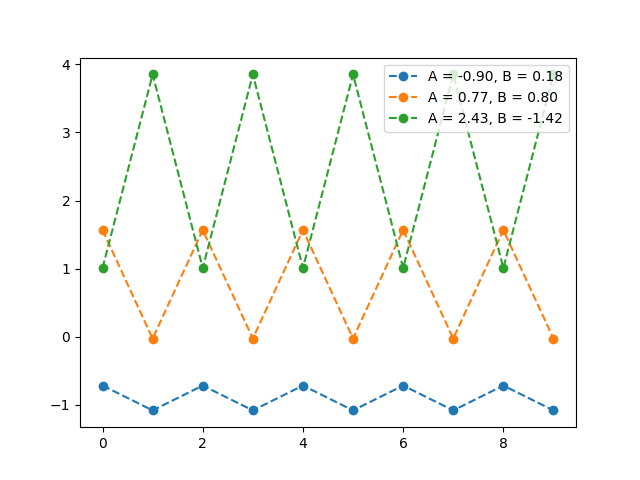
\includegraphics[width=0.9\textwidth]{gfx/33_fig.png}
\label{fig1}
\caption{Beispiele wie $A+(-1)^tB$ ausschauen kann.}
\end{figure}

%34
\item Für welche der folgenden Folgen folgt positive Semidefinitheit definitiv aus ihrer Definition? Wann gilt Stationarität? Plots!
\begin{enumerate}
%a
\item $a_k := \begin{cases}
1 & k = 0 \\
0.8 & k \in \{-1, 1\} \\
0 & \text{sonst}
\end{cases}$
\begin{align*}
\end{align*}

%b
\item $b_k := 1$
\begin{align*}
\end{align*}

%c
\item $c_k := \begin{cases}
-0.25 & k = -1 \\
1 & k = 0 \\
0.25 & k = 1 \\
0 & \text{sonst}
\end{cases}$
\begin{align*}
\end{align*}

%d
\item $d_k := 1.25^{|k|}$
\begin{align*}
\end{align*}
\end{enumerate}

\begin{figure}[h!]
\centering
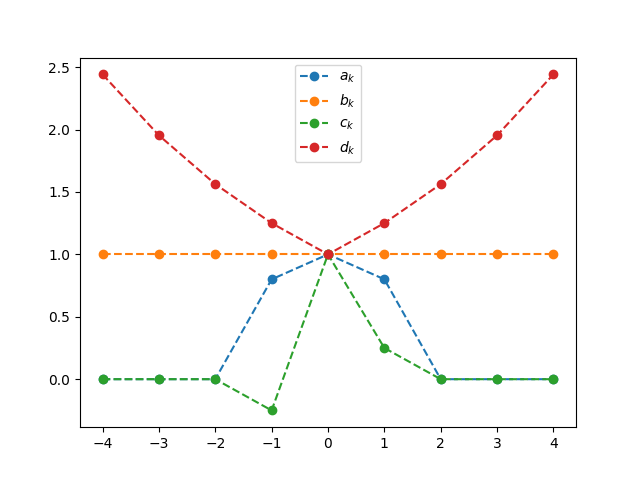
\includegraphics[width=0.9\textwidth]{gfx/34_fig.png}
\label{fig2}
\caption{Die betrachteten Folgen.}
\end{figure}


\end{enumerate}
\end{document}
